\documentclass[tikz,11pt]{beamer}
\usepackage[utf8]{inputenc}
\usepackage[T1]{fontenc}
\usetheme{default}
\usepackage{lipsum}
\usepackage{listings}

% ----------------------------
% fabio - headers
% ----------------------------

\usepackage{tikz}
\usetikzlibrary{matrix,arrows.meta}

\begin{document}
    \begin{frame}
	\frametitle{Objetivos do Trabalho}
	
	O objetivo principal do trabalho foram:
	
	\begin{itemize}
		\item Estudar a estrutura e o funcionamento de Redes Neurais
		Convolucionais 2D
		\item Entender como a informação é transformada dentro da
		rede neural ao avançar nas camadas mais profundas
		\item Extrapolar esse conhecimento para redes mais
		clássicas como a \textbf{MLP} estudada durante a
		disciplina.
	\end{itemize}
	\end{frame}

\begin{frame}
	\frametitle{Introdução e Motivação}
\end{frame}

\begin{frame}
	\frametitle{Apresentação do Bruno}
\end{frame}

\begin{frame}
	\frametitle{Apresentação do Bruno Canale}
\end{frame}

\begin{frame}
	\frametitle{Python - Keras Framework para Machine Learning}
	
	* Python - Linguagem de programação gratuita \newline
	* Contém uma quantidade muito grande de Frameworks voltados para
	\textit{Machine Learning}
	
	
	\begin{figure}
		\centering
		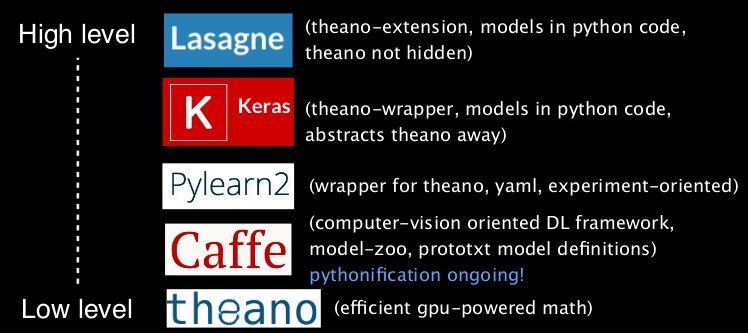
\includegraphics[scale=0.3]{road_map}
	\end{figure}
	
	Keras foi inicialmente desenvolvido como parte de um projeto de
	pesquisa chamado de ONEIROS (Open-ended Neuro-Electronic
	Intelligent Robot Operating System)
	
\end{frame}

\begin{frame}
	\frametitle{Keras - Exemplo de implementação MLP}
	
	
	modelo = Sequential() \\
	modelo.add(Dense(num-neuronios, init='uniform'))\\
	modelo.add(Activation('tanh')) \newline
	
	modelo.add(Dense(1, init='uniform')) \\
	modelo.add(Activation('linear')) \newline
	
	modelo.compile(learning-rate=0.1, optimizer='sgd]') \newline
	
	modelo.fit(features-treino, target-treino) \newline
	
	modelo.predict(features-teste)
	
\end{frame} 

\begin{frame}
	\frametitle{Base de dados utilizada - MNIST}
	
	\begin{columns}
		\begin{column}{0.48\textwidth}
			A base de dados MNIST é composta por 60.000 exemplos de
			imagens de digitos em letra cursivas. O dataset é ideal para
			testes de algoritmos em reconhecimentos de padrões por
			necessitar pouco pré-processamento.\\
			Mais informações no link: http://yann.lecun.com/exdb/mnist/
		\end{column}
		\begin{column}{0.48\textwidth}
			\begin{figure}
				\centering
				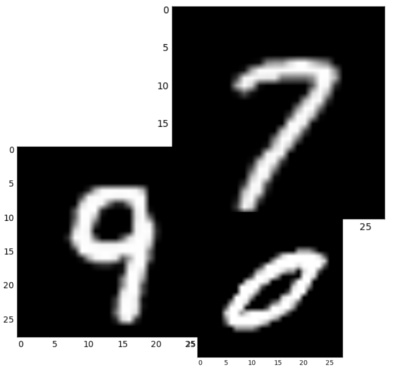
\includegraphics[scale=0.35]{minst}
			\end{figure}
		\end{column}
	\end{columns}
	
	\lstinputlisting[language=Python, firstline=0, lastline=10,
	basicstyle=\ttfamily\scriptsize]{base_import.py}
\end{frame}

\begin{frame}
	\frametitle{Processamento necessário no atributo target}
	
	Um processamento padrão é transformar o conjunto de
	\textbf{atributos targets} em um conjunto de variáveis
	categóricas. O que seriam variáveis categoricas?
	
	Exemplo: Se a lista de targets é composta por: [1.2, 2, 3, 4.2,
	4i] e as classes disponiveis são \textbf{real, inteiro,
		imaginario}, então uma matriz de transformação seria:
	
	\begin{table}[h]
		\caption{Conversão para variáveis categoricas}
		\begin{tabular}{l|c|c|c|}
			
			target & real & inteiro & imaginario \\
			1.2    & 1    & 0       & 0 \\
			2      & 0    & 1       & 0 \\
			3      & 0    & 1       & 0 \\
			4.2    & 1    & 0       & 0 \\
			4i     & 0    & 0       & 1
			
		\end{tabular}
	\end{table}
\end{frame}

\begin{frame}
	\frametitle{Implementação da Rede Convolucional 2D}
	\lstinputlisting[language=Python, firstline=0, lastline=25,
	basicstyle=\ttfamily\scriptsize]{cnn1.py}
\end{frame}

\begin{frame}
	\frametitle{Modelo do Experimento realizado para análise da
		Rede}
	\begin{itemize}
		\item Após implementação a arquitetura foi testada para
		verificar performance no conjunto de testes.
		\item Queriamos observar a transformação da imagem de Input
		após cada camada da ConvNet
		\item A fim de analisar com mais detalhes, foram adicionadas
		mais camadas convolucionais no modelo apresentado anteriormente.
	\end{itemize}
\end{frame}

% -------------------------------------------------
% \begin{fabio}
% -------------------------------------------------

\begin{frame}
	\frametitle{Redes e Resultados}

    \begin{figure}
	\centering
	\begin{minipage}{.33\textwidth}
		\centering
		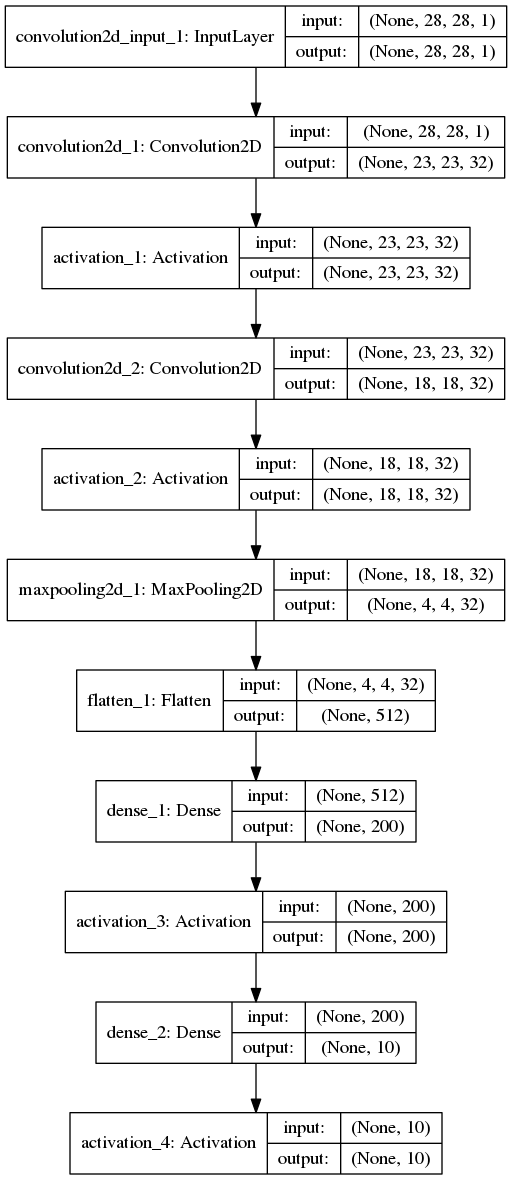
\includegraphics[width=.4\linewidth]{images/resultados/default/model}
	\end{minipage}%
	\begin{minipage}{.33\textwidth}
		\centering
		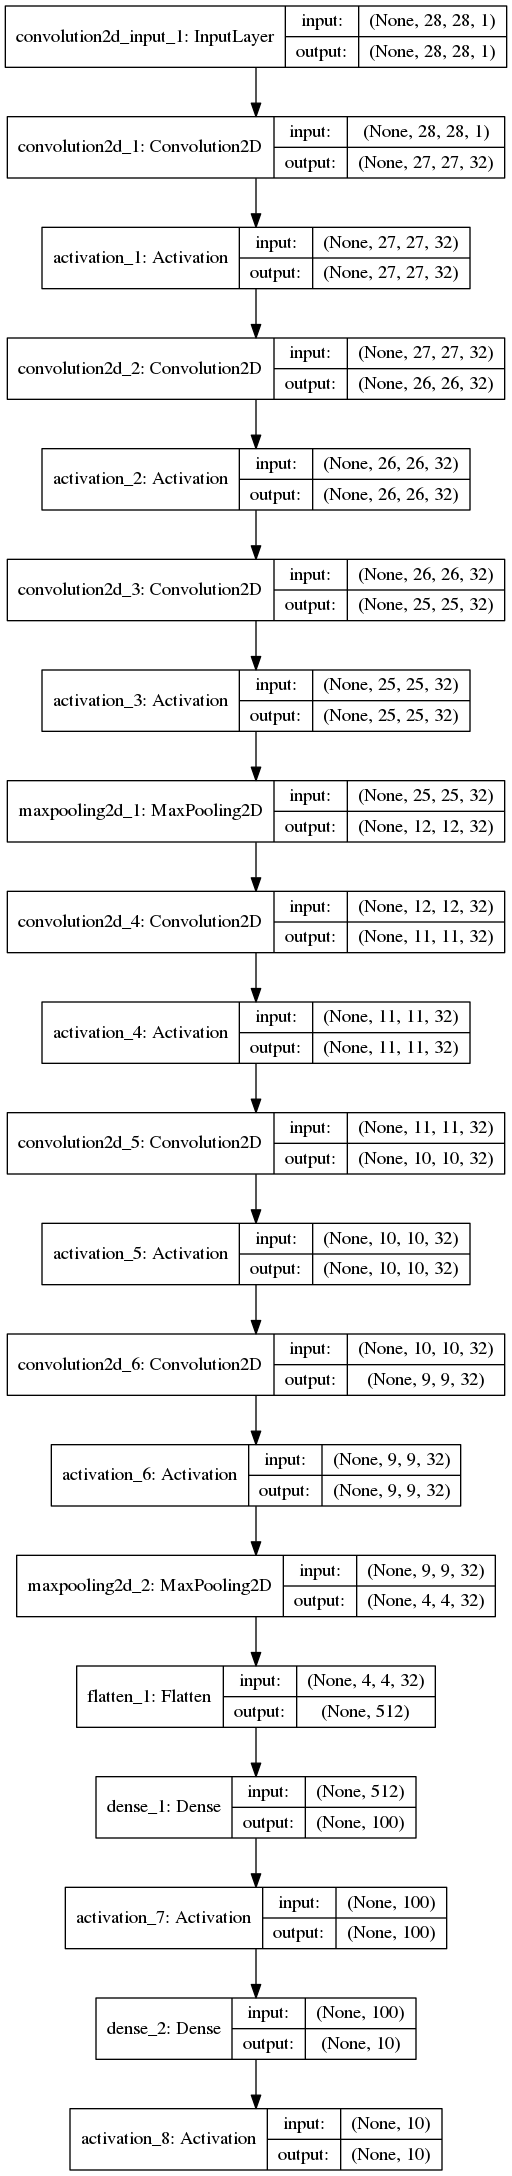
\includegraphics[width=.4\linewidth, height=.9\textheight]{images/resultados/network_1/model}
	\end{minipage}%
	\begin{minipage}{.34\textwidth}
	\centering
	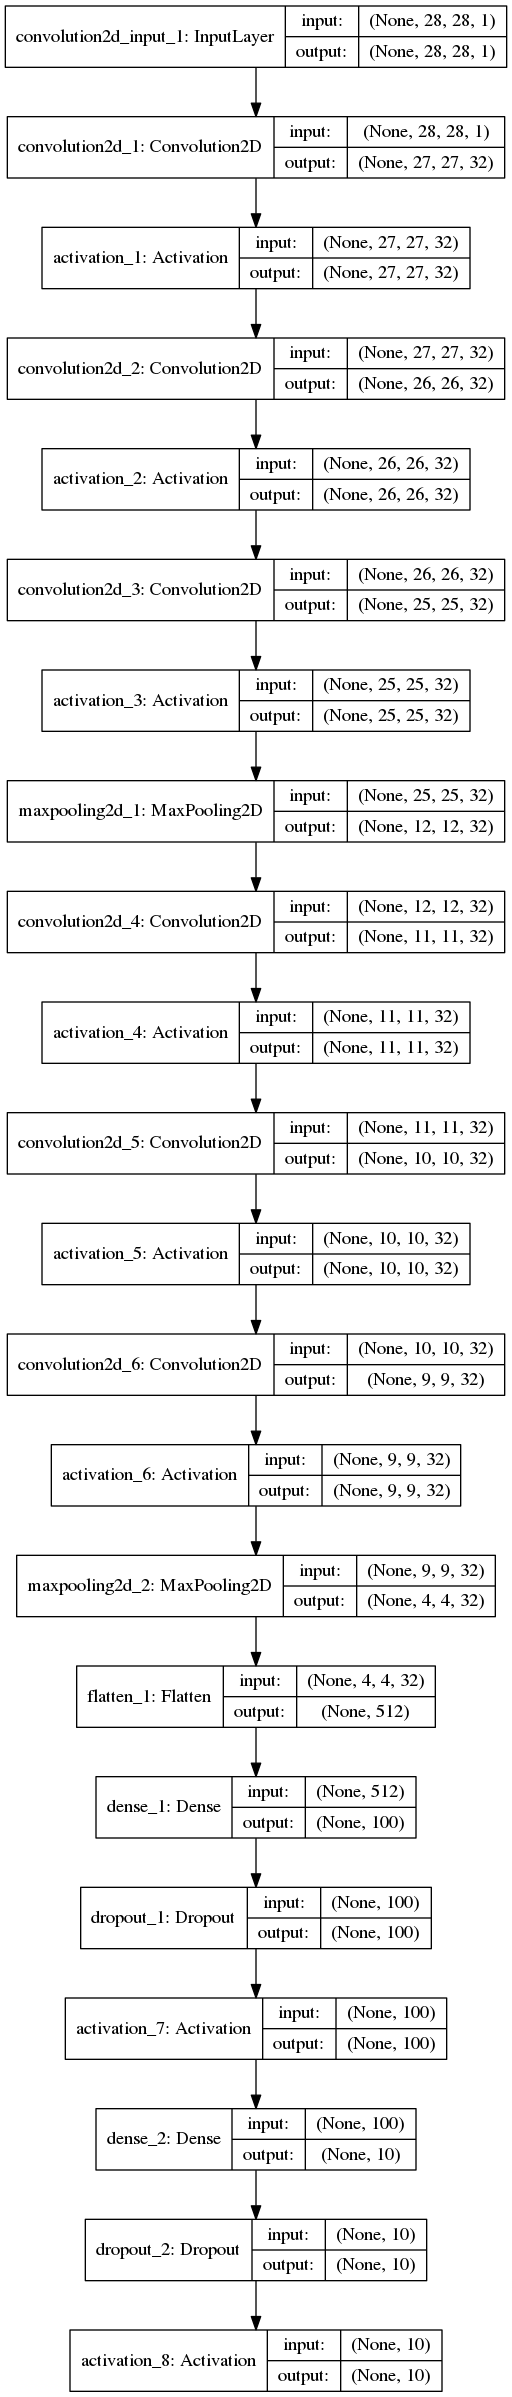
\includegraphics[width=.4\linewidth, height=.9\textheight]{images/resultados/network_2/model}
	\end{minipage}

\end{figure}

\end{frame}


\begin{frame}
	\frametitle{Camada de entrada}
	\centering
	MNIST DATASET
	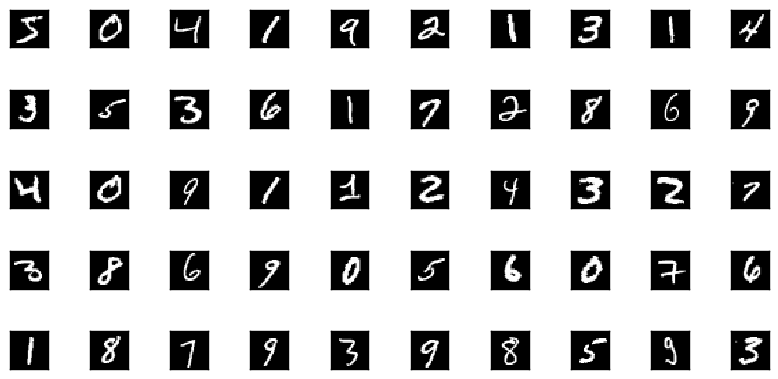
\includegraphics[width=.8\paperwidth]{images/fabio/inputs}
\end{frame}

\begin{frame}
	\frametitle{Aplicação da CNN}
	\centering
	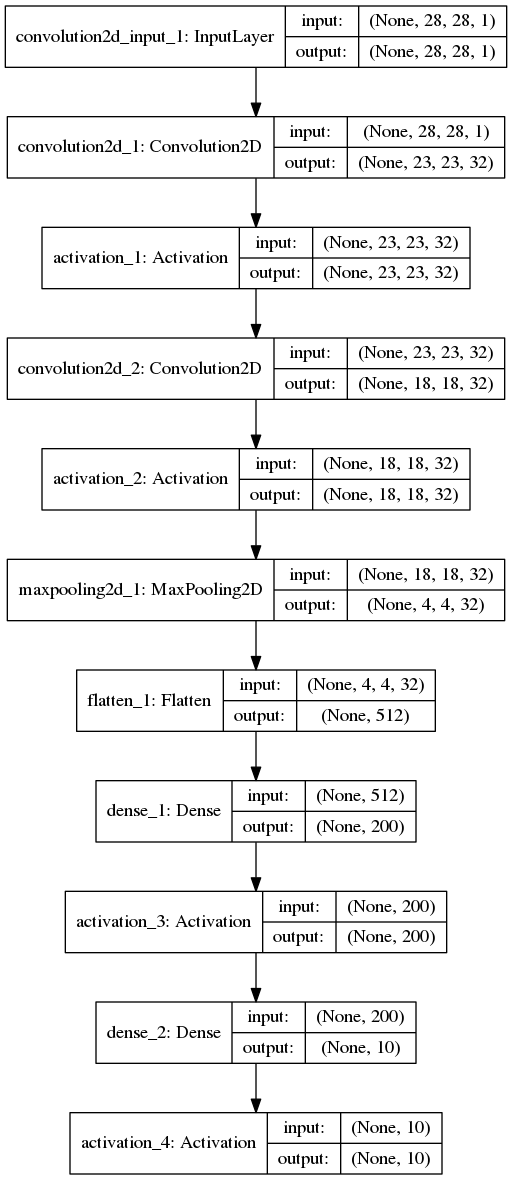
\includegraphics[height=.8\paperheight]{images/resultados/default/model}
\end{frame}

\begin{frame}
	\frametitle{Treinamento}
	\centering
%	\begin{minipage}{.5\textwidth}
		\centering
		\par Treinamento
		\begin{itemize}
			\item Épocas = 10
			\item Itens = 60000
			\item Tempo = 30 ~ 40 minutos
		\end{itemize}		
%	\end{minipage}%
%	\begin{minipage}{.5\textwidth}
	\centering
	\par Teste
	\begin{itemize}
		\item Itens = 10000
	\end{itemize}		
	\centering
	\par Resultado na base de teste
	\begin{itemize}
		\item 98.02\%
	\end{itemize}
%\end{minipage}%

\end{frame}

\begin{frame}
	\frametitle{Convolução - 1}
	\centering
	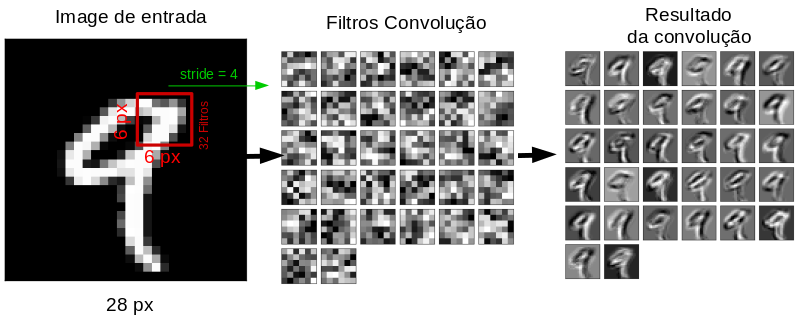
\includegraphics[width=.8\paperwidth]{images/fabio/conv_1}
\end{frame}

\begin{frame}
	\frametitle{Ativação - 1}
	\centering
	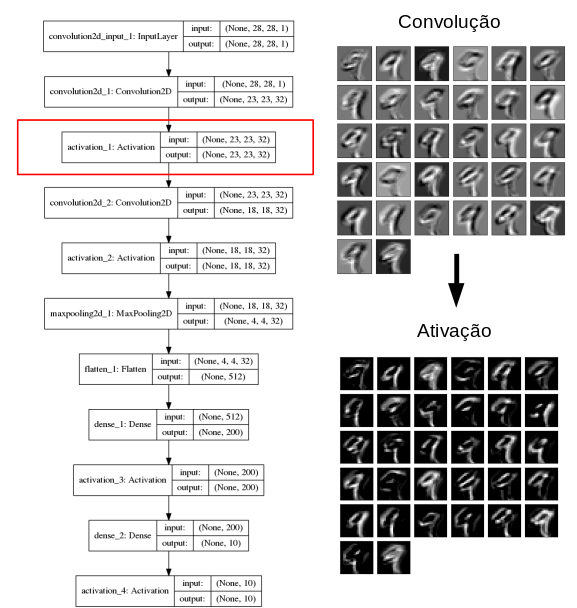
\includegraphics[height=.8\paperheight]{images/fabio/ativ_1}
\end{frame}

\begin{frame}
	\frametitle{Convolução - 2}
	\centering
	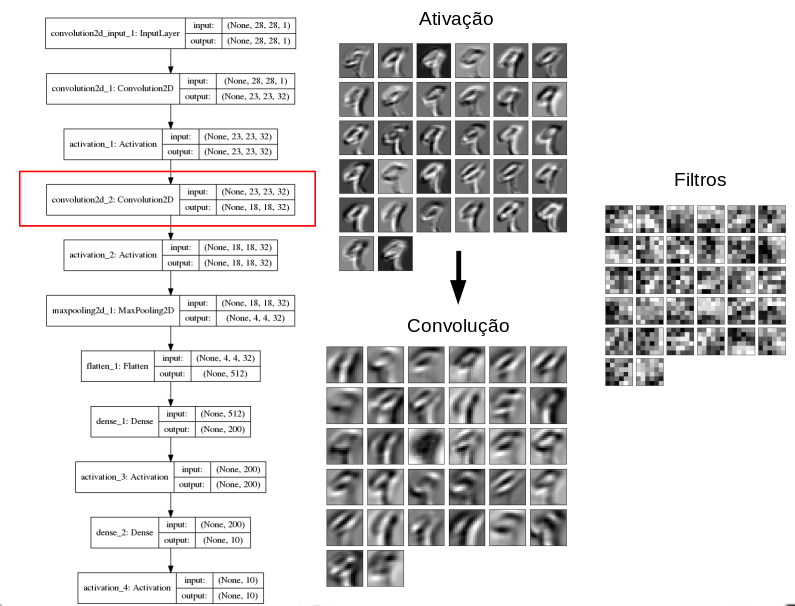
\includegraphics[width=.8\paperwidth]{images/fabio/conv_2}
\end{frame}

\begin{frame}
	\frametitle{Ativação - 2}
	\centering
	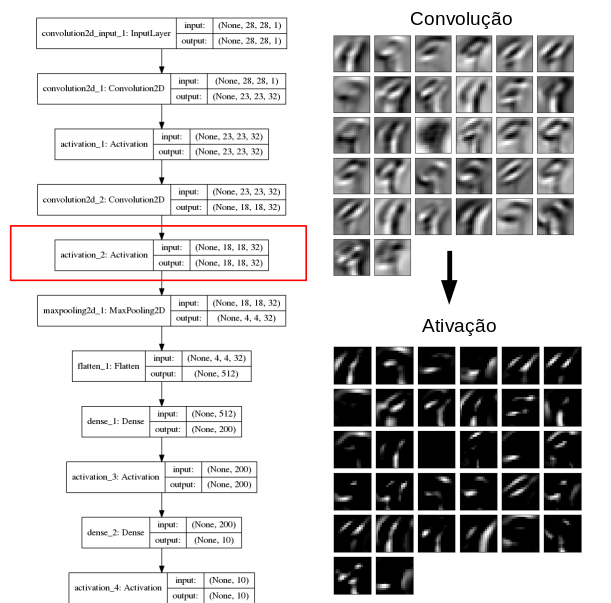
\includegraphics[height=.8\paperheight]{images/fabio/ativ_2}
\end{frame}

\begin{frame}
	\frametitle{Pooling}
	\centering
	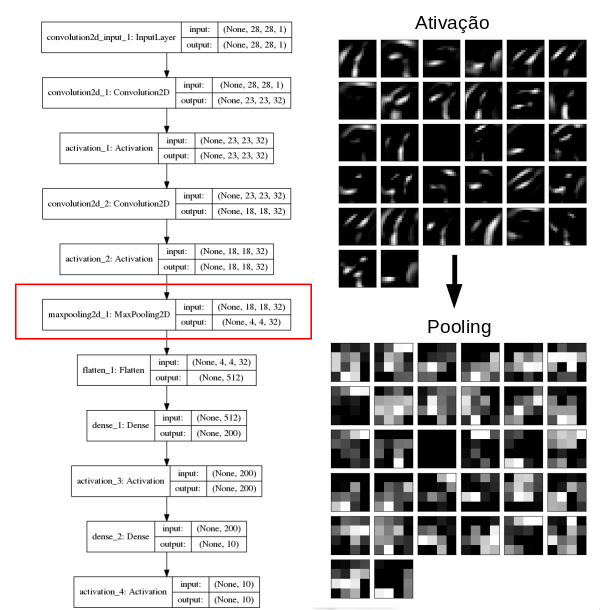
\includegraphics[height=.8\paperheight]{images/fabio/pooling_1}
\end{frame}

\begin{frame}
	\frametitle{Flatten ( N * 2D -> 1D)}
	\centering
	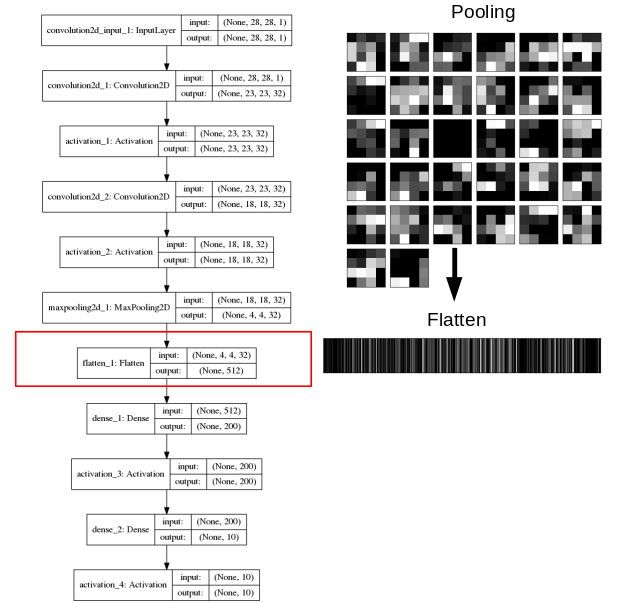
\includegraphics[height=.8\paperheight]{images/fabio/flatten_1}
\end{frame}


\begin{frame}
	\frametitle{Dense - 1}
	\centering
	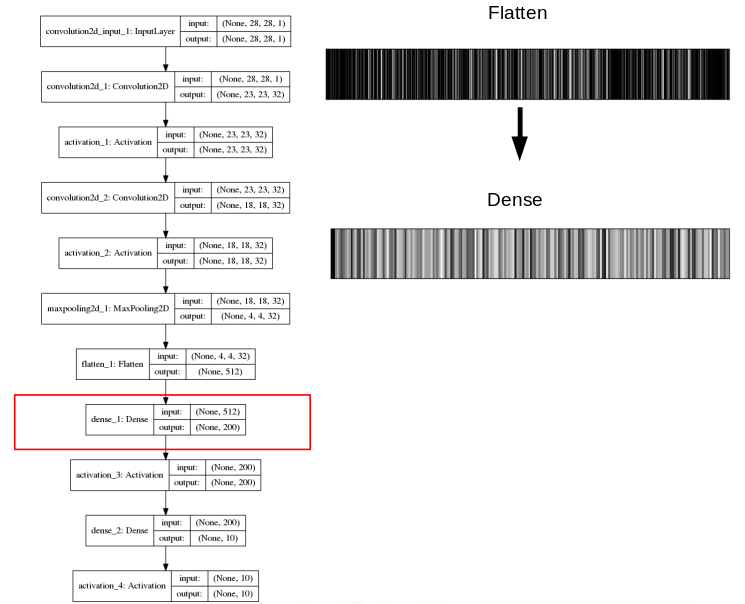
\includegraphics[height=.8\paperheight]{images/fabio/dense1}
\end{frame}

\begin{frame}
	\frametitle{Ativação - 3}
	\centering
	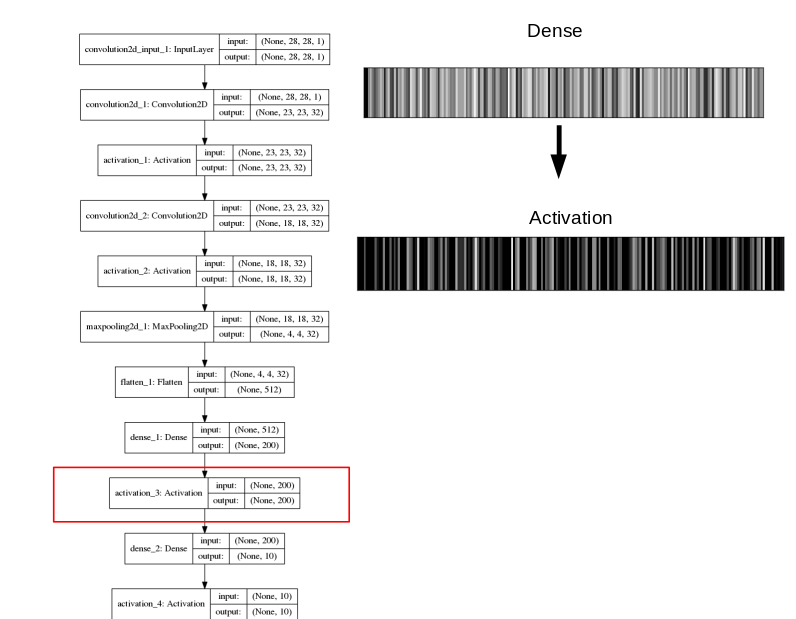
\includegraphics[height=.8\paperheight]{images/fabio/ativ_3}
\end{frame}

\begin{frame}
	\frametitle{Dense - 2}
	\centering
	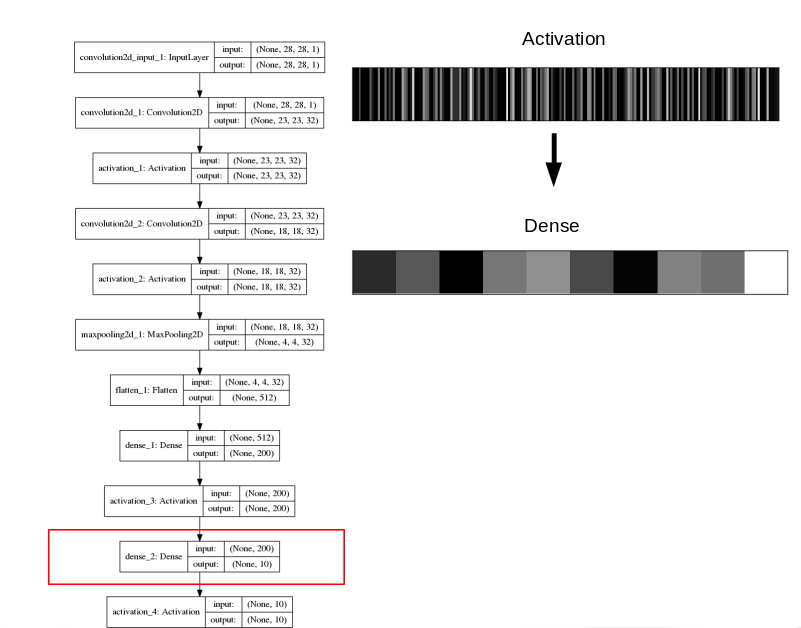
\includegraphics[height=.8\paperheight]{images/fabio/dense2}
\end{frame}

\begin{frame}
	\frametitle{Ativação - 4}
	\centering
	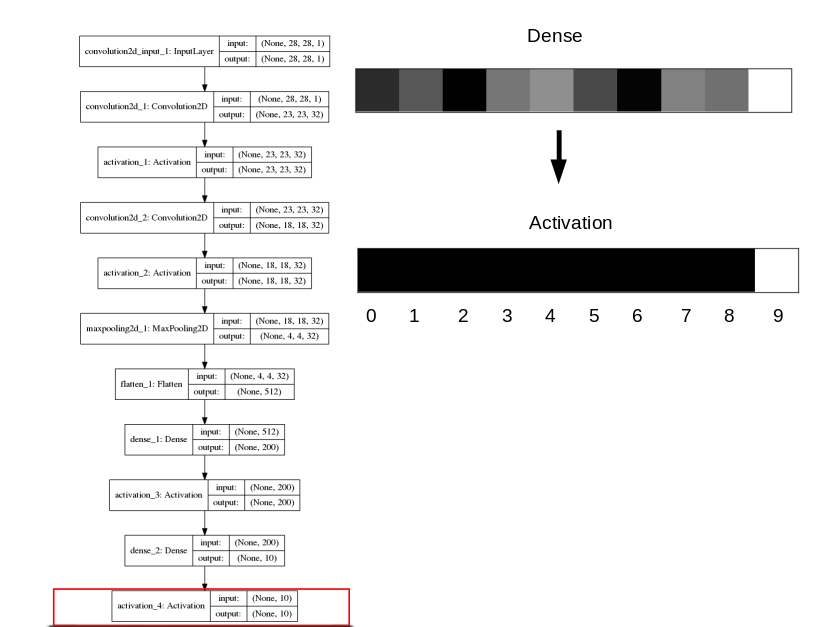
\includegraphics[height=.8\paperheight]{images/fabio/ativ_4}
\end{frame}


\begin{frame}
	\frametitle{Resultados das demais redes testadas - 1 }
	\centering
	\par Precisão na base de treino: 98.94\%
	\par Precisão na base de teste: 98.89\%
	\par 3 conv + 1 pooling + 3 conv + 1 pooling + 2 FC 
	\\
	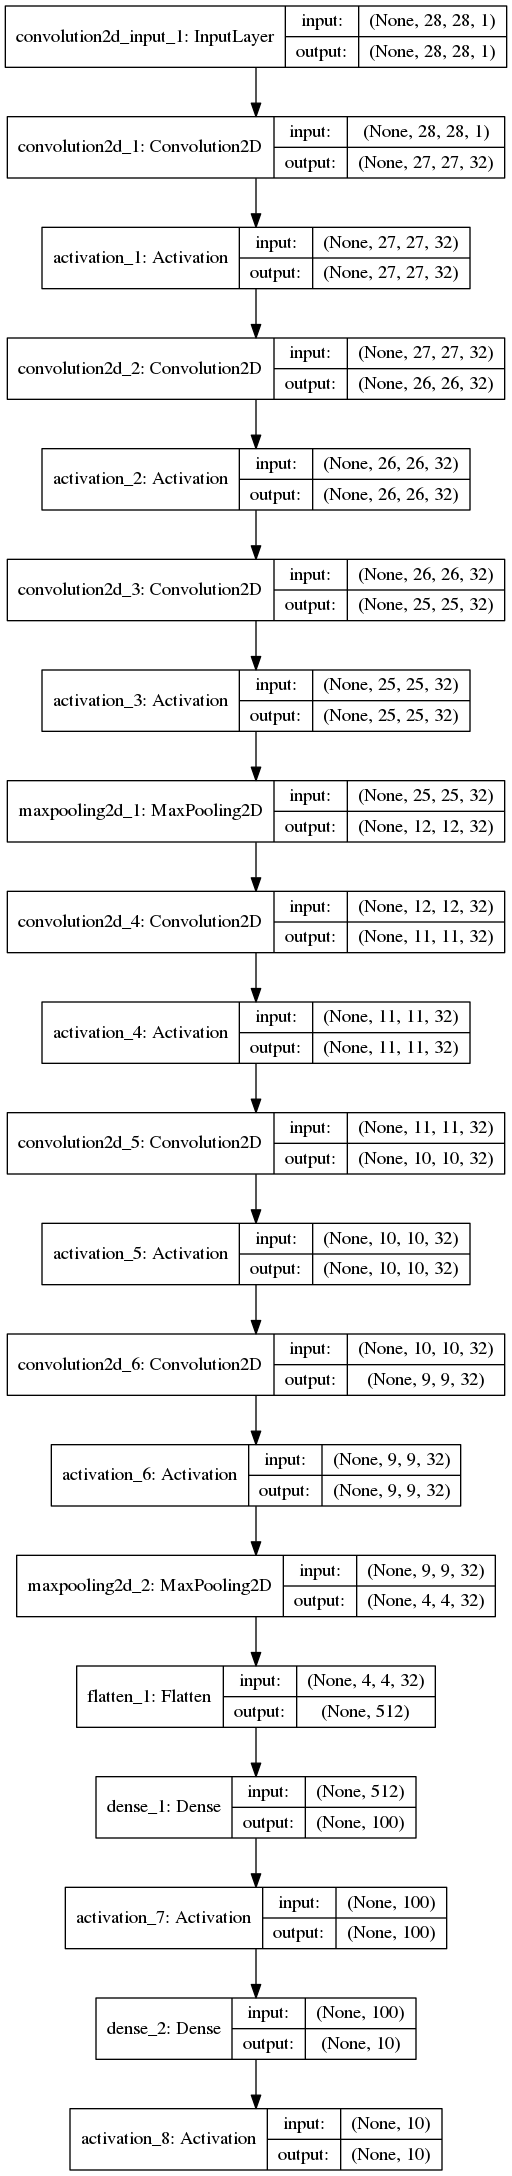
\includegraphics[height=.7\paperheight]{images/resultados/network_1/model}
\end{frame}

\begin{frame}
	\frametitle{Resultados das demais redes testadas - 2 }
	\centering
	\par Precisão na base de treino: 98.94\%
	\par Precisão na base de teste: 99.06\%
	\par 3 conv + 1 pooling + 3 conv + 1 pooling + 2 FC \(com dropout\)
	\\
	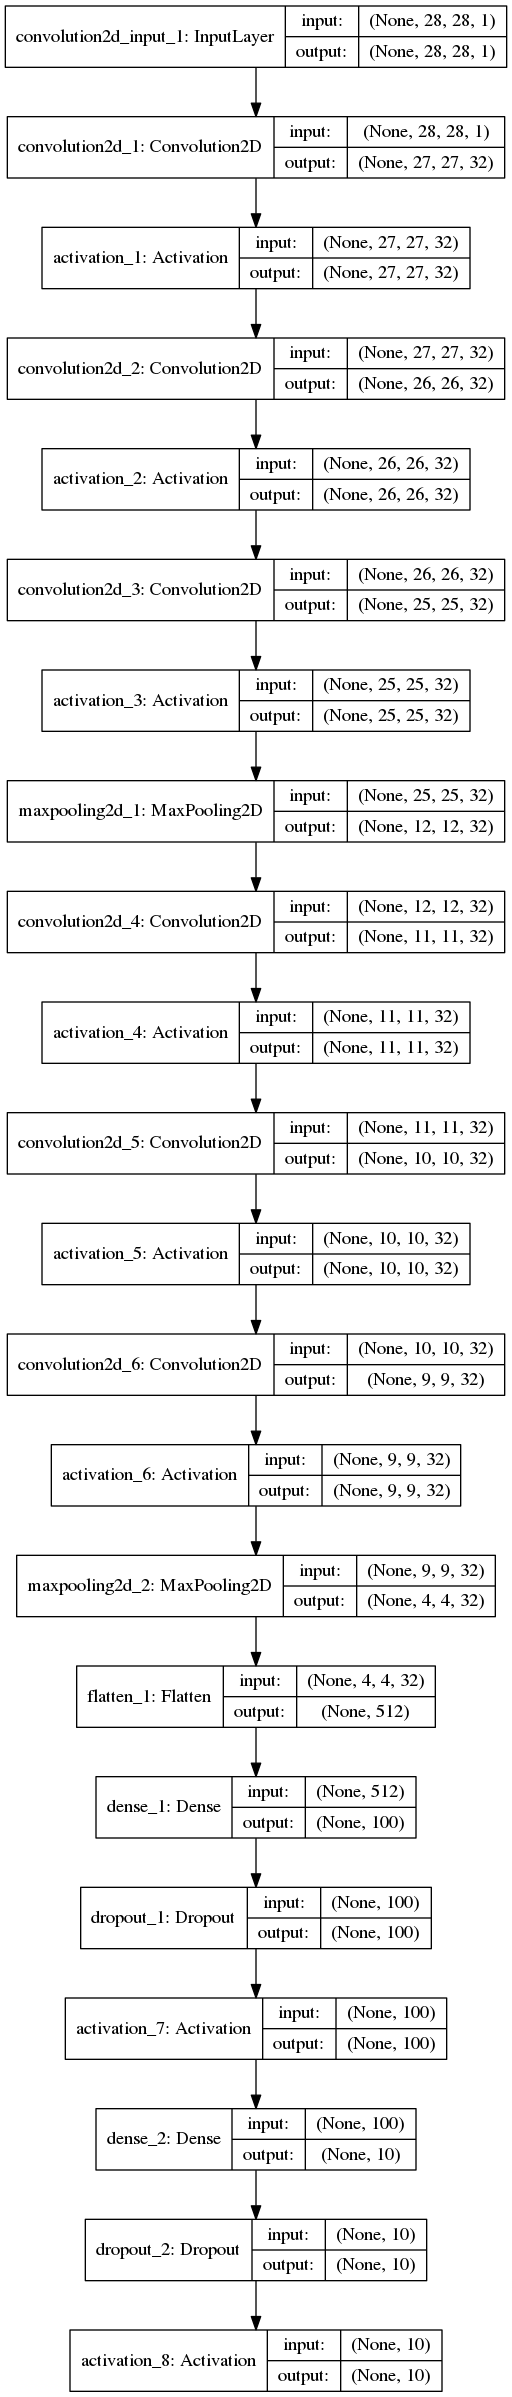
\includegraphics[height=.7\paperheight]{images/resultados/network_2/model}
\end{frame}

\begin{frame}
	\frametitle{MLP \& CNN}
	\centering
	\begin{itemize}
		\item CNN é uma extensão do conceito da MLP
		\item Convoluções e Pooling ajudam a diminuir rapidamente o número de variáveis do sistema
		\item Próprio para o processamento de imagens e vídeos		
	\end{itemize}
\end{frame}

% -------------------------------------------------
% end{fabio}
% -------------------------------------------------
\end{document}